% document formatting
\documentclass[10pt]{article}
\usepackage[utf8]{inputenc}
\usepackage[left=1in,right=1in,top=1in,bottom=1in]{geometry}
\usepackage[T1]{fontenc}
\usepackage{xcolor}
\usepackage[table,xcdraw]{xcolor}

% math symbols, etc.
\usepackage{amsmath, amsfonts, amssymb, amsthm}

% lists
\usepackage{enumerate}
\usepackage{tabularx}

% images
\usepackage{graphicx} % for images
\usepackage{tikz}

% code blocks
\usepackage{minted, listings} 

% verbatim greek
\usepackage{alphabeta}

\graphicspath{{./assets/images/Week 1}}

\title{03-621 Week 1 \\ \large{Advanced Quantative Genetics}}
 
\author{Aidan Jan}

\date{\today}

\begin{document}
\maketitle

\section*{Genetics in the Post-Genome Era}
\begin{itemize}
    \item Late 1990s: First large genomes sequenced (\textit{Saccharomyces cerevisiae, Drosophila melanogaster})
    \item 2001: First draft of the human genome sequence
    \item Now: Sequenced genomes of many different organisms and thousands of individual humans
\end{itemize}
The goal now that we have the entire human genome documented are to:
\begin{itemize}
    \item Identify the genes (defined by sequence) that control traits of interest
    \item Identify the functions of specific genes or DNA sequences
    \item Understand regulatory and functional relationships among genes
    \item Develop safe or efficient methods of Genome Engineering
    \item Personalized treatments, gene therapy, and early diagnosis
\end{itemize}

\subsection*{What is the Human Genome?}
The human genome is the \textbf{complete set} of genetic information found in our cells.
\begin{itemize}
    \item Nuclear: 
    \begin{itemize}
        \item $3 \times 10^9$ base pair (bp) DNA organized as large linear fragments in chromosomes, including
        \begin{itemize}
            \item 22 autosomes
            \item X and Y sex chromosomes (XX female, XY male)
        \end{itemize}   
        \item Low gene density
        \begin{itemize}
            \item $\sim 20000$ protein-coding genes
            \item $\sim 23000$ RNA genes
            \item Functional significance of \textbf{most} of the nuclear genome remains a mystery
        \end{itemize}   
    \end{itemize}
    \item Mitochondrial:
    \begin{itemize}
        \item $16.6 \times 10^3$ base pairs of circular DNA (many copies) 
        \begin{itemize}
            \item inherited from mother only
        \end{itemize}
        \item High gene density
        \begin{itemize}
	        \item 13 protein-coding genes (for oxidative phosphorylation)
	        \item 2 rRNA genes (for translation of mitochondrial mRNAs)
	        \item 22 tRNA genes (for translation of mitochondrial mRNAs)
        \end{itemize}
    \end{itemize}
\end{itemize}

\subsection*{Nuclear Genome}
\begin{itemize}
	\item Contained in the nucleus of every cell
	\item 23 chromosomes total for humans
	\item Have areas of low and high gene density (e.g., not equally distributed)
\end{itemize}
Cells in Diploid organisms contain two copies of the genetic material organized as pairs of \textbf{homologous chromosomes}.
\begin{itemize}
	\item Non-gamete cells have $2n = 46$ (23 pairs) of chromosomes
	\item Gametes have $1n = 23$ pairs.
\end{itemize}
\begin{center} 
	\includegraphics*[width=0.5\textwidth]{W1_1.png} 
\end{center}

\subsection*{Mitochondrial Genome}
\begin{itemize}
	\item Origin of Mitochondria: prokaryotic endosymbiont
	\item High compaction: little non-coding space
	\item Only two transcription units: from P$_H$ and P$_L$ (opposite strands)
	\item The two large transcripts are cleaved into smaller RNAs for translation
\end{itemize}
\begin{center} 
	\includegraphics*[width=0.5\textwidth]{W1_2.png} 
\end{center}

\section*{What is a Gene?}
\begin{itemize}
	\item \textbf{Genetic definition:} a gene is a unit of inheritance transmitted from parent to offspring.
	\begin{itemize}
	    \item A given gene can exist in different forms (alleles: sequence variants) that can influence a trait (i.e., a characteristic) of the organism (e.g., blue vs. brown eyes).
    \end{itemize}
    \item \textbf{Molecular definition:} genes are specific segments (DNA sequences) in chromosomes that are transcribed to produce:
    \begin{itemize}
        \item protein-coding RNA (mRNA)
        \item non-protein-coding coding RNA:
        \begin{itemize}
	        \item RNAs involved in translation (rRNAs, tRNAs)
	        \item Regulatory RNAs (e.g., miRNAs, siRNAs, piRNAs, IncRNAs)
        \end{itemize}
    \end{itemize}
\end{itemize}

\subsection*{Structure of a Typical Protein-coding Eukaryotic Gene}
\begin{center} 
	\includegraphics*[width=\textwidth]{W1_3.png} 
\end{center}

\section*{Gregor Mendel}
He defined basic laws of inheritance for all eukaryotes.\\\\
Why did he succeed?
\begin{itemize}
	\item It was easy to cross defined strains with his chosen organism (pea plants)
	\item He chose obvious and distinct traits!
	\item He used pure-breeding lines so that the genetic constitutions were reproducible
\end{itemize}

\subsection*{Pure Breeding Lines}
\begin{itemize}
	\item Genes can come in different versions, called \textbf{alleles}
	\item All plants of a pure-breeding line are identical in terms of their inheritance determinants.
\end{itemize}
\begin{center} 
	\includegraphics*[width=0.5\textwidth]{W1_4.png} 
\end{center}

\subsection*{Particulate Inheritance}
A theory that states that genetic determinants behave like particles and are inherited as discrete units (the alleles of genes) without blending\\\\
For example, for Mendel's round and wrinkled peas (alleles \textit{R} and \textit{r})
\begin{itemize}
	\item In the parental generation, he cross-breeded true-breeding Round and wrinkled strains.  (\textit{RR} $\times$ \textit{rr}).
	\item In the F1 generation, all the phenotypes were round since the genotypes of all the plants was heterozygous (\textit{Rr}).
	\item Cross-breeding the F1 plants resulted in both round strains and wrinkled strains, in a three-to-one ratio.
\end{itemize}
The alleles that come together in a cross between two individuals can be separated and recovered in \textit{equal frequency} in crosses of their progeny.
\begin{center} 
	\includegraphics*[width=0.4\textwidth]{W1_5.png} 
\end{center}

\subsection*{Definitions}
\begin{itemize}
	\item The parental trait that is expressed in the monohybrid F1 is called \textbf{dominant}
	\item The parental trait that is latent in the monohybrid F1 is called \textbf{recessive}
	\item A \textbf{Homozygous} individual is one with two identical alleles of the gene of interest, such as \textit{RR} or \textit{rr}.
	\item A \textbf{Heterozygous} individual is one with two different alleles of the gene of interest, such as \textit{Rr}.
	\item The \textbf{Punnett Square} is the mathematical model we use for tracking alleles.  (see above)
\end{itemize}

\subsection*{Dihybrid Cross}
What if we are following inheritance of two traits at once?  For example, Mendel's pea shape and color.
\begin{center} 
	\includegraphics*[width=0.8\textwidth]{W1_6.png} 
\end{center}
Note that this is the result \textit{only} if the genes are unlinked: different chromosomes, or far apart on the same chromosome.

\subsection*{Important Chromosome Nomenclature}
\begin{center} 
	\includegraphics*[width=\textwidth]{W1_7.png} 
\end{center}

\subsection*{Why Gametes are Unique}
First, the difference between mitosis and meiosis.  For reference, $n$ is the number of chromosomes, and $c$ is the number of copies of the DNA.
\begin{itemize}
	\item Both processes start with a diploid mother cell. (2n)
	\item Mitosis separates sister centromeres.  First, chromosomes are duplicated (2n, 4c), then divided into two cells.  As a result, the two resulting cells have the same genetic information. (2n, 2c)
	\item In Meiosis, there are two stages.
	\begin{itemize}
	    \item In Meiosis I, homologous non-sister centromeres are separated. (1n, 2c)
	    \item In Meiosis II, sister centromeres are separated, similar to Mitosis. (1n, 4c)
	    \item As a result, there are four daughter cells, and they have different genetic information
    \end{itemize}
\end{itemize}
Diploid cells have two copies of the DNA (2n), and haploid cells have one copy (1n).  All somatic cells are diploid, and all gametes (sex cells) are haploid.\\\\
When gametes are formed, there are two things that make them unique.
\begin{enumerate}
	\item \textbf{Independent Assortment:} since each gamete only contains one copy of DNA, the copy from the original pair of chromosomes it inherits is randomized.  Since there are 23 chromosomes for humans, and each chromosome comes in a pair, there are a total of $2^{23}$ different possible gametes from independent assortment.
	\item \textbf{Crossing Over:} For each pair of chromosomes, during the first meiosis stage, the two chromosomes can switch sections with each other at random locations.  As a result, two genes on the same chromosome are more likely to be inherited together the closer their location on the chromosome is, since the less likely they will be separated during this stage.
\end{enumerate}
\subsubsection*{Crossing Over}
\begin{center} 
	\includegraphics*[width=\textwidth]{W1_8.png} 
\end{center}

\section*{Complementation}
Suppose we have a species of flower with multiple strains.  Blue flowers are dominant, and white flowers are recessive.  Let all the strains here be true breeding.
\begin{itemize}
	\item If we cross breed a blue flower with a white flower, the F1 generation would be all blue (heterozygous), and the F2 generation would have blue and white, in a 3:1 ratio.  This is expected.
	\item However, we find out that crossing two white flowers also yields an all-blue F1 generation, and inbreeding the F1 generation leads to a F2 generation with blue and white flowers, in a 9:7 ratio.  How is this possible?
\end{itemize}
\textbf{Complementation} occurs when recessive variants with the same phenotype are not alleles of the same genes.  In this case, suppose color is controlled by two genes, A and B.
\begin{itemize}
	\item For flowers to be blue, they must have dominant alleles in both of them.  Therefore, the one white flower may have AAbb, and the other may have aaBB.  Both are white since both have one recessive pair.
	\item When cross-breeding, all the children (F1) are heterozygotes (AaBb).  Therefore, all of them are blue.
	\item Inbreeding these flowers result in a 9:7 ratio of blue to white flowers.
\end{itemize}
\begin{center}
\begin{tabularx}{7cm}{|>{\centering\arraybackslash}X|>{\centering\arraybackslash}X|>{\centering\arraybackslash}X|>{\centering\arraybackslash}X|>{\centering\arraybackslash}X|}
\hline
\rule{0pt}{0.5cm} &  AB & Ab & aB & ab \\ \hline
\rule{0pt}{0.5cm}AB & \cellcolor[HTML]{34CDF9}AABB & \cellcolor[HTML]{34CDF9}AABb & \cellcolor[HTML]{34CDF9}AaBB & \cellcolor[HTML]{34CDF9}AaBb \\ \hline
\rule{0pt}{0.5cm}Ab & \cellcolor[HTML]{34CDF9}AABb & AAbb & \cellcolor[HTML]{34CDF9}AaBb & Aabb \\ \hline
\rule{0pt}{0.5cm}aB & \cellcolor[HTML]{34CDF9}AaBB & \cellcolor[HTML]{34CDF9}AaBb & aaBB & aaBb \\ \hline
\rule{0pt}{0.5cm}ab & \cellcolor[HTML]{34CDF9}AaBb & Aabb & aaBb & aabb \\ \hline
\end{tabularx}
\end{center}

\subsection*{How do we interpret complementation?}
Suppose flowers need to express a pigment protein to be blue.  We may have a system like
\begin{center}
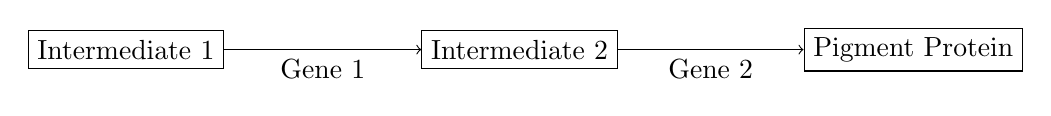
\begin{tikzpicture}
    \node[draw] at (0, 0) (a) {Intermediate 1};
    \node[draw] at (5, 0) (b) {Intermediate 2};
    \node[draw] at (10, 0) (c) {Pigment Protein};

    \draw[->] (a) to node[below] {Gene 1} (b);
    \draw[->] (b) to node[below] {Gene 2} (c);
\end{tikzpicture}
\end{center}
Therefore, both genes must have at least one dominant allele for the flower to be blue.\\\\
Alternatively, we may also have the system
\begin{center}
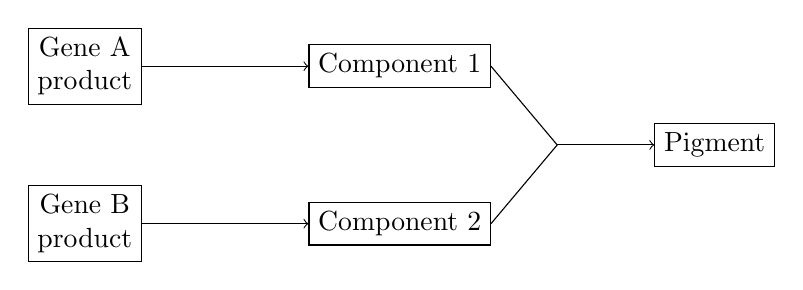
\begin{tikzpicture}
    \node[draw, align=center] at (0, 2) (a1) {Gene A\\product};
    \node[draw, align=center] at (0, 0) (b1) {Gene B\\product};
    \node[draw] at (4, 2) (a2) {Component 1};
    \node[draw] at (4, 0) (b2) {Component 2};
    \node[draw] at (8, 1) (c) {Pigment};
    
    \coordinate (t) at (6, 1);

    \draw[->] (a1) edge (a2);
    \draw[->] (b1) edge (b2);
    \draw (a2.east) -- (t) -- (b2.east);
    
    \draw[->] (t) -- (c);
\end{tikzpicture}
\end{center}
The ability to recognize complementation is very important for understanding the genetic basis of human traits and heritable disorders.
\begin{itemize}
	\item Complementation allows us to classify each recessive mutation into a particular ``complementation group'': a set of recessive alleles with similar phenotypes that DO NOT complement one another.
	\item Each \textbf{complementation group} defines a \textbf{functional unit} that may be an entire gene, or an element \textit{within} a gene that can function independently of others (a cell-specific transcription enhancer; an alternatively spliced exon; a protein domain \dots)
\end{itemize}
Human genetic diseases with the \textbf{same phenotype} very often arise from mutations in \textit{different genes}.  (E.g., Xeroderma pigmentosum, or hypersensitivity to the sun)

\subsection*{Complementation Tests}
\begin{itemize}
	\item Standard tool used with model experimental organisms
	\item Mutagenesis and genetic screens can be performed to identify mutations in \textbf{all} genes that potentially affect a particular biological process
\end{itemize}
\begin{center} 
	\includegraphics*[width=0.6\textwidth]{W1_9.png} 
\end{center}

\end{document}